\documentclass{llncs}

\usepackage[american]{babel}
\usepackage{graphicx}
\usepackage[T1]{fontenc}

\usepackage[
bookmarks=false,
breaklinks=true,
colorlinks=true,
linkcolor=black,
citecolor=black,
urlcolor=black,
pdfpagelayout=SinglePage
]{hyperref}
% enables correct jumping to figures when referencing
% \usepackage[all]{hypcap}

% to typeset URLs, URIs, and DOIs
\usepackage{url}
\def\UrlFont{\rmfamily}
\usepackage{epstopdf}
\usepackage[]{subfig}
\usepackage{amsmath}
\usepackage{bm}
\usepackage{amssymb}

\usepackage{bbding}


\begin{document}

\title{Efficient Algebraic Multigrid Preconditioners \\on Clusters of GPUs}
%
%\titlerunning{Hamiltonian Mechanics}  % abbreviated title (for running head)
%                                     also used for the TOC unless
%                                     \toctitle is used
%
\author{Ambra Abdullahi Hassan\inst{1}%
\and Valeria Cardellini\inst{1} \and Pasqua D'Ambra\inst{2} \and \\ 
Daniela di Serafino\inst{3} \and  Salvatore Filippone\inst{4}}
%
%\authorrunning{} % abbreviated author list (for running head)
%
\institute{Universit\`a degli Studi di Roma ``Tor Vergata'', Roma, Italy\\
 \email{\{ambra.abdullahi,cardellini\}@uniroma2.it}
\and
Istituto per le Applicazioni del Calcolo ``Mauro Picone'', CNR, Napoli, Italy\\
 \email{pasqua.dambra@cnr.it}
\and
Universit\`a degli Studi della Campania ``Luigi Vanvitelli'', Caserta, Italy
\email{daniela.diserafino@unicampania.it}
\and
 Cranfield University, Cranfield, UK\\
 \email{salvatore.filippone@cranfield.ac.uk}
}
\maketitle              % typeset the title of the contribution

\begin{abstract}
Many scientific applications require the solution of large and sparse linear systems of equations using iterative methods, this operation accounting for a large percentage of the computing time. In these cases, the choice of the preconditioner is crucial for the convergence of the iterative method.
Given the broad range of applications, great effort has been put in the development of efficient  preconditioners ensuring algorithmic scalability: in this sense, multigrid methods have been proved to be particularly promising.
Additionally, the advent of GPUs, now found in many of the fastest supercomputers, poses the problem of implementing efficiently these algorithms on highly parallel architectures; this is made more difficult by the fact that the solution of sparse triangular systems, a common kernel in many types of preconditioners, is extremely inefficient on GPUs. 

In this paper, we use the PSBLAS and MLD2P4 libraries to explore various issues that affect the efficiency of multilevel preconditioners on GPUs, both in terms of execution speed and exploitation of computational cores, as well as the algorithmic efficiency in guaranteeing convergence to solution in a number of iterations independent of the parallelism degree. 
We investigate these issues 
%are investigated 
in the context of linear systems arising from groundwater modeling application of the filtration of 3D incompressible single-phase flows through %anisotropic 
porous media.

\end{abstract}
%
\section{Introduction}

Many engineering and scientific applications often require the solution of
linear systems
 \begin{equation}
 Ax = b, \qquad x,b \in \Bbb{R}^n,\, A\in \Bbb{R}^{n\times n},
\label{eq:linsys}
\end{equation}
where the matrix $A$ is large and sparse. In our context, \emph{large}
means millions or even billions of unknowns, whereas
\emph{sparse} means that most coefficients in $A$ are zero and it is
convenient to employ special storage formats. In many applications,
and specifically in the test cases discussed in this paper, the matrix
$A$ is also symmetric and positive definite. 

The solution of such systems is achieved by using either direct or iterative methods. 
However, for large and sparse linear systems, direct methods are  difficult to implement in parallel
because of their recursive nature and often suffer from high computational complexity~\cite{Templates}.  
Therefore, a more viable alternative is to use iterative solvers and Krylov
subspace methods are the most widely used class of these solvers~\cite{MR1990645}. 
%The most widely used solvers for systems of this type are Krylov subspace methods~\cite{MR1990645}.
Their time to solution is determined by the number
of iterations performed and by the time per iteration, and hence their 
efficiency is the result of a tradeoff between iteration complexity and speed of convergence. 
A critical feature is the application of preconditioning,
corresponding, e.g., to a transformation of the form
\begin{equation}\label{eq:preclinsys}
M^{-1}Ax=M^{-1}b,
\end{equation} 
which is aimed at speeding up the convergence of Krylov methods through the improvement of
the ``quality'' of the system matrix. Note that the
product $M^{-1}A$ is not computed explicitly, but the Krylov solvers
are modified so that it is obtained by performing at each iteration
the computation of $M^{-1} v$, where $v$ is a suitable vector. 

Multigrid methods are widely used as preconditioners, because they are optimal,
in the sense that their computational cost grows linearly with the number of unknowns
when the linear systems come from the discretization of elliptic partial differential
equations~\cite{Vassilevski2008}.
Many efforts have been performed to extend their efficiency
to more general systems, often the direction of a complete
algebraic approach, where no information on the origin of the problem
is exploited. In this case, they are called Algebraic MultiGrid (AMG) methods~\cite{Stuben2001}.

The linear complexity of AMG preconditioners generally
translates into algorithmic scalability, i.e., the number of iterations
of AMG-preconditioned Krylov solvers does not depend on the size of the
problem. This allows efficient parallel implementations on multiple CPUs,
for example through a domain decomposition approach, in which rows of
the matrix are assigned to different computing nodes.
The diffusion of General Purpose Graphics Processing Units (GPGPUs),
currently found in many of the fastest supercomputers on the Top 500 list
(\url{https://www.top500.org/lists/}), requires the exposition of a high
degree of parallelism, because GPUs are high-throughput many-core processors.
Since AMG methods are obtained by combining different components (smoother,
coarsening algorithm, coarsest-level solver, restriction and prolongation operators),
a full exploitation of GPU capabilities requires each component to be optimized
for this type of architecture.

In this work, we focus on the choice and implementation of AMG smoothers
and coarsest-level solvers capable of harnessing the computational power offered by
a cluster of GPUs. We consider block-Jacobi smoothers and solvers that use sparse
approximate inverses to perform the local solves required by each block, instead of typical
incomplete factorization methods. The choice of sparse approximate inverses
is motivated by the much larger amount of parallelism exposed by
sparse matrix-vector products as compared to the parallelism available
in sparse triangular solves. Furthermore, suitable implementations of sparse approximate
inverse preconditioners have already proved their efficiency on a single GPU (see, e.g.,
\cite{BERTACCINI2016693,Lukash:2012}). 
In our work, the smoothers and local solvers are used within
the AMG framework offered by the MLD2P4 package of preconditioners~\cite{mld-toms} 
and exploiting sparse matrix data structures and Krylov solvers from
the PSBLAS  library~\cite{PSBLAS3}. 
We conducted an extensive set of weak scalability tests on the JURECA supercomputer at the J\"ulich Supercomputing Centre (JSC), 
using a groundwater modelling application developed at JSC. 
To quantify the gain in efficiency and performance using the cluster of GPUs, we also ran tests only on CPUs. 
Our results show scalability up to 128 GPUs and 256 millions equations.

%and are analyzed in terms of both execution speed and algorithmic scalability.
To the best of our knowledge, the selected AMG smoothers and local solvers have not been
considered in other AMG preconditioners tailored for GPUs~\cite{BellDaltonOlson:2012, }. 

%\textbf{Aggiungere biblio:
%Bell, Dalton, Olson; Park, Smelianskiy, Yang, ...; Rupp, Weinbub}. 

Furthermore, most results have been so far presented on a single GPU; 
for example, Richter et al.~\cite{Richter:2014} presented the implementation for discrete elliptic field problems 
using the CUSP library. 

In this work, we do not consider the setup phase of the preconditioner,
which will be the subject of future work. 
Of course, an efficient AMG setup on multiple GPUs is important for the overall efficiency of the
preconditioner. Nevertheless, in situations where we need to solve multiple
linear systems with the same coefficient matrix, it is desirable to obtain
the best possible efficiency during the solution phase even at the expense of a
longer setup time, because this will be amortized over multiple
solution steps.

The remainder of this article is organized as follows. In Section~\ref{AMG} we briefly describe AMG preconditioners,
identifying their main sparse matrix kernels. In Section~\ref{SLA-GPU}, we discuss the main issues
concerning the implementation of these kernels on GPUs. In Section~\ref{results} we illustrate the
behaviour of the AMG preconditioners on a cluster of GPUs on linear systems coming from a
a groundwater modelling applications. 
We conclude in Section~\ref{sec:concl} with some final remarks.  
%

\section{Algebraic Multigrid Preconditioners\label{AMG}}
%
%MultiGrid methods are widely used as preconditioners of iterative
%Krylov solver for sparse linear systems. 
%They are very efficient methods, having linear computational
%complexity and hence perfect scalability, when 
%sparse and large linear systems stemming
%from the discretization of some scalar elliptic Partial Differential
%Equations (PDEs) have to be solved~\cite{Vassilevski2008}. 
%Many efforts are related to extend their efficient applicability also
%to more general systems, in particular in the direction of a complete
%algebraic approach, where no information on a possible geometric
%origin of the problem is exploited. In this last case, they are called
%Algebraic MultiGrid (AMG) or Algebraic Multilevel
%methods~\cite{Stuben2001}. 
Multigrid methods achieve  their efficiency by the recursive application
of two complementary processes: \emph{relaxation} and \emph{coarse-grid
correction}.
%
\begin{figure}[t]
\begin{center}
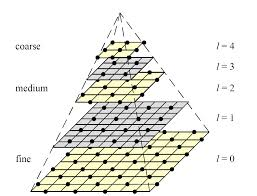
\includegraphics[width=.75\textwidth]{multilevel.png}
\caption{A MultiGrid hierarchy.\label{hierarchy}}
\end{center}
\end{figure}
%
Relaxation consists in the application of an iterative method, such as
Jacobi or Gauss-Seidel, to reduce highly oscillatory error components,
while the coarse-grid correction corresponds to the solution of the
resulting residual equation in an appropriately chosen coarse space,
aimed at reducing the leftover error components. The recursive application
of this procedure leads to a \emph{multilevel hierarchy} of spaces,
depicted in Fig.~\ref{hierarchy}. 

In the classical multigrid approach, the coarser grid and the interpolation
operator for transferring the coarse-grid solution to the original (fine) grid are
predefined by the geometry of the problem. Conversely,
AMG methods address the setup phase, known as~\emph{coarsening process},
in an automatic way, without using explicit knowledge of the
problem which the linear system originates from, and relying only on the entries of
the system matrix. Here we consider
an algebraic coarsening process based on the aggregation strategy,
where coarse-grid unknowns are aggregates of original
unknowns. In particular, the AMG preconditioners available in the MLD2P4
library~\cite{mld-toms} rely
on a decoupled version of \emph{the smoothed aggregation} algorithm
described in~\cite{BrezinaVanek96,BrezinaVanek99}. This procedure is
currently implemented on the host CPUs; for the sake of space,
we refer the reader to~\cite{mld2p4-2-guide} for details on the related
algorithm and its parallel implementation.

Our aim here is to identify the main linear algebra
operations needed for the application of the AMG preconditioner with
a Krylov solver, since the efficient implementation of these operations on
GPUs is the main focus of this work. 

The application phase of an AMG preconditioner is also known as
multigrid cycle. The most widely used one is the so called symmetric
V-cycle, described in Fig.~\ref{Vcycle}, where the AMG hierarchies of
$nlev$ prolongator operators $P^k$ and of corresponding coarse
matrices, obtained by the standard variational approach
$A^{k+1}=(P^{k+1})^TA^kP^{k+1}$, have been built in the setup phase.
%
\begin{figure}[t]
\begin{center}
\framebox{
\begin{minipage}{.85\textwidth}
\begin{tabbing}
\quad \=\quad \=\quad \=\quad \\[-3mm]
procedure V-cycle$\left(k,A^k,b^k,x^k\right)$ \\[2mm]
\>if $\left(k \ne nlev \right)$ then \\[1mm]
\>\> $x^k = x^k + (M^k)^{-1} \left(b^k - A^k x^k\right)$ \\[1mm]
\>\> $b^{k+1} = (P^{k+1})^T\left(b^k - A^k x^k\right)$ \\[1mm]
\>\> $x^{k+1} =$ V-cycle$\left(k+1,A^{k+1},b^{k+1},0\right)$ \\[1mm]
\>\> $x^k = x^k + P^{k+1} x^{k+1}$ \\[1mm]
\>\> $x^k = x^k + (M^k)^{-T} \left(b^k - A^k x^k\right)$ \\[1mm]
\>else \\[1mm]
\>\> $x^k = \left(A^k\right)^{-1} b^k$\\[1mm]
\>endif \\[1mm]
\>return $x^k$ \\[1mm]
end
\end{tabbing}
\end{minipage}
}
\caption{V-cycle preconditioner.\label{Vcycle}}
\end{center}
\end{figure}
%
$M^k$ represents the matrix
operator corresponding to the basic iterative method applied as smoother
at level $k$. 

The main computational kernels in the application of the preconditioner
are the sparse matrix-vector multiplication and the inversion of  $M^k$.
In the simple case of Jacobi method, $M^k=diag(A^k)$ and hence
inverting $M^k$ corresponds to a highly parallel vector
update operation. On the other hand, more robust iterative methods,
such as the Gauss-Seidel method or incomplete factorizations, are
often required to improve the convergence of the preconditioned solver
applied to general linear systems. In these cases, the inversion of
the corresponding matrix operators requires the solution of triangular
systems, which is a sequential kernel. Therefore, an
efficient parallel implementation of the V-cycle is
strictly related to the availability of iterative
methods which can be formulated in terms of sparse matrix-vector multiplication (SpMV)
and, possibly, vector updates, and to an efficient implementation of the sparse
matrix-vector multiplication.


%
\section{Sparse Linear Algebra and Preconditioners on GPUs}

General Purpose Graphics Processing Units (GPGPUs)~\cite{Luebke06}  
are today an established and attractive choice in the world of
scientific computing, found in many among the fastest supercomputers
on the Top~500 list, and offered in standard Cloud infrastructure
services, e.g. in  Amazon EC2. It is therefore not surprising that
they are at the focus of many research efforts revolving around the
efficient implementation of scientific software, including solvers for
sparse linear system of equations. 

Many applications use iterative methods to solve sparse linear
systems;  the most popular ones are those based on  Krylov subspace 
projection methods~\cite{MR1990645}. 

From a  software point of view, all Krylov methods employ the matrix $A$ 
to perform matrix-vector products  $y\gets Ax$, whose efficient
implementation provides significant challenges on all modern computer
architectures. 
The SpMV kernel is well-known to be a memory-bounded application;
and  its bandwidth usage  is strongly dependent on both the input
matrix and on the underlying computing platform(s). For a detailed
overview of the implementation issues and a survey of available
techniques for this kernel on GPUs, see~\cite{Filippone:2017:SMM:3034774.3017994}.   

For most real-world problems,it is necessary to combine the Krylov
solvers with  \emph{preconditioners}. A preconditioner is a
transformation applied to the coefficient  matrix such that the
resulting linear system has better convergence properties. Examples of
popular preconditioners include Jacobi and Gauss-Seidel iterations,
Block Jacobi and Additive Schwarz coupled with incomplete
factorizations,  and Algebraic Multigrid. 

To implement a linear system solver on a parallel computing
architecture, we typically use a \emph{domain decomposition} approach,
in which subsets of the computational domain are assigned to different
computing nodes. Domain decomposition requires to achieve a number of
trade-offs among multiple factors:
\begin{itemize}
\item Many preconditioners, e.g. Gauss-Seidel or incomplete
  factorizations, employ kernels for the solution to sparse triangular
  systems; in using sparse triangular solvers, we normally  want the
  sparsity pattern to be of the same order as that of the original
  coefficient matrix;
\item However, the amount of parallelism available in a sparse
  triangular solution is dependent on the number of nonzeros in the
  sparse factors, and is usually very small;
\item To overcome this issue, most preconditioners use a Block Jacobi
  or hybrid Gauss-Seidel strategy, in which the sparse triangular
  solve is used only within the local subdomain, while employing a
  global Jacobi-like correction;
\item Unfortunately, the convergence properties of these local schemes
  deteriorate with increased parallelism.
\end{itemize}
The last phenomenon is often described as a loss of \emph{algorithmic
  scalability}, i.e., the ability to obtain a convergence history that
is independent of the degree of parallelism. In summary, simple
preconditioning schemes, such as Point Jacobi, have good algorithmic scalability,
because their convergence properties do not change much with an
increasing number of processes, but the more sophisticated
Gauss-Seidel and incomplete factorizations are a lot more efficient in
serial computations. 

Multilevel corrections, or Algebraic Multigrid  preconditioners, offer
a way to recover algorithmic scalability: 
it is possible to apply efficient local approximate solvers, while a
good convergence history is recovered by relying on the multilevel
corrections. 

Finding the preconditioning combination that gives the best overall
performance is thus a very complex enterprise. In this context, the
ability to combine multiple options in a flexible framework such as
the one we described in~\cite{mld-toms} is an essential ingredient. 

Additional considerations are necessary when implementing
preconditioning operations on GPUs. First of all, implementing the
solution of sparse triangular systems on GPUs is extremely difficult.
As an example, the conjugate gradient preconditioned with incomplete
LU available in CUDA CuSPARSE since version 4.0~\cite{Naumov11}
achieves at best a speedup factor of about 2 over a standard CPU
implementation. The main reason is that the GPU requires a massive
amount of data parallelism to be exploited, and in the sparse
triangular factors the amount of available parallelism is limited by
the sparsity. 
The two main  options that  are available  involve the use of
matrix-vector products as their main kernel:
\begin{itemize}
\item Point-Jacobi iterations; 
\item (Local) preconditioning through sparse approximation of the
  inverses.
\end{itemize}
For a discussion of sparse approximate inverses on GPUs 
see~\cite{BERTACCINI2016693}. 


The implementation of the multilevel preconditioners for which we will
present results in this paper is based on MLD2P4~\cite{mld-toms} and
PSBLAS~\cite{psblas3}. Thanks to the modular architecture of both
packages, it is possible to define \emph{plugins} for 
\begin{itemize}
\item Operators on the GPU, including sparse matrix-vector product
  supporting multiple storage formats and vector-vector operations;
\item Approximate inverses as local solvers.
\end{itemize}
By combining these ingredients in a multilevel framework we can obtain
interesting scalability results. 

Three additional practical obstacles must be mentioned here. 
First of all, the preconditioner is invoked at least once per
iteration of the Krylov method.  Because the allocation of memory
on the GPU is an expennse synchronization point, this means that the
memory space for internal work areas must be preallocated for all
invocations  of the preconditioner; allocation of auxiliary data areas at
each invocation of the prevonditioner is perfectly doable on the CPU
side, but leads to a slowdown by a factor of 2 on the GPU. 

The second issue has to do with the implementation of the
matrix-vector product on the GPU: as mentioned
in~\cite{Filippone:2017:SMM:3034774.3017994}, the most effective
storage formats are often derived from ELLPACK  and assign one thread
per row of the matrix; this means that to exploit a GPU it is
necessary to have matrices which are sufficiently large to keep all
computing units busy, and this is very difficult at the coarse level
of the preconditioner hierarchy because the size of the aggregates is
small. Indeed, it may be convenient to limit the number of levels to
be less than the default that would be used in a normal CPU
implementation. 
{\bf DA VERIFICARE CON I DATI DI PERFORMANCE}. 

The third issue is related to the efficiency of communication between
the various computing nodes; to proceed with the computation of the
matrix-vector product in parallel between the different nodes, it is
necessary to exchange the data of the \emph{halo}. For good data
partitions, the amount of data to be exchanged displays a
surface-to-volume effect, and therefore large products can be computed
effectively; however when moving between different levels of the
preconditioning hierarchy we are precisely going towards smaller
matrices, hence the surface-to-volume ratio and the efficiency of the
parallelization decreases. The speed ratio of the GPU with respect to
the CPU only makes things worse; again, it may be necessary to limit
the number of levels to less than what would be efficient when using
CPUs. 
% \section{Sparse linear algebra on GPUs}
% Sparse linear algebra on GPU e limitazioni del nucleo risoluzione di sistemi triangolari, uso delle inverse approssimate e focus sulla INVK di PSBLAS.
\section{Results\label{results}}

We illustrate the behaviour of the MG preconditioner for GPUs described so far,
which exploits the INVK sparse approximate inverse solver. This approximate
inverse is obtained by the inversion of triangular
factors based on a positional drop strategy~\cite{vanDuin:99,BERTACCINI2016693}.
In particular, we show the results obtained on a linear system
arisen from a groundwater modelling application developed at the
J\"ulich Supercomputing Centre (JSC), concerning the numerical simulation
of the filtration of 3D incompressible single-phase flows through
anisotropic porous media. It is an elliptic equation with no flow
boundary conditions;  the linear systems stem from the discretization
of the equation performed by a cell-centered finite column scheme
(two-point flux approximation) on a Cartesian grid, with nonzero
entries distributed over seven diagonals. In these tests, we will
consider a homogeneous permeability tensor;  this application comes
from the framework of the Horizon 2020 EoCoE Project (Grant
676629). The equations are discretized over the unit cube; the
computational domain is partitioned by repeated sectioning along
coordinate planes. 

We performed weak scalability tests using approximately 2 millions
equations per process; thus  the total dimension ranges from 2
millions up to 256 millions equations. 

The experiments were performed on  the JURECA supercomputer at JSC.
Each GPU compute node consists
of two NVIDIA Tesla K80 GPUs with a dual-GPU design, for a total of
four available GPU devices per compute nodes.   
We used PSBLAS 3.5 (combined with its extension plugin for extended
matrix formats and GPU plugin) and MLD2P4 2.1 (combined with AINV
plugin),  compiled with  GNU compilers (C and Fortran) version 5.4.0,
MVAPICH2 version 2.3 and with CUDA 8.0.61. 

The linear systems are solved using the Conjugated Gradient (CG) method.
The stopping criterion is based on the ratio between the 2-norms of the
residual and the right-hand side vectors: the method halts if this ratio becomes smaller than $10^{-6}$).
CG is used in conjunction with a V-cycle preconditioner, for
which we consider two different configurations. In the first case the
V-cycle preconditioner applies, as pre- and post-smoother, 1 sweep of
the block-Jacobi method with INVK as a solver. In the
second configuration it applies, as pre- and post-smoother,, 2 sweep
of the Jacobi solver. In both cases, we use 10 sweeps of Block Jacobi with INVK  as
coarsest level solver.   The multilevel hierarchy is built with a
decoupled smoothed aggregation algorithm. 

For each configuration, we ran tests on CPUs only, with matrices in
CSR format, and using CPUs+GPUs, with matrices in ELLPACK format. This
allows us to quantify the gain in efficiency in using GPUs.   


\begin{figure}
\begin{center}
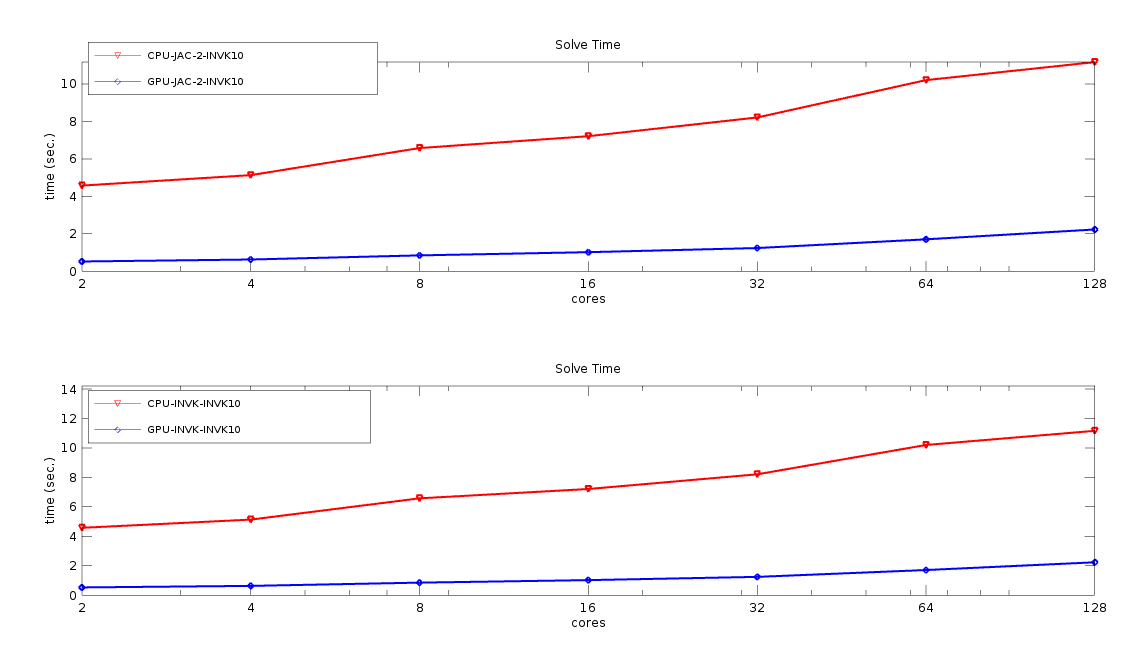
\includegraphics[width=\textwidth]{graf_solve_1.png}
\end{center}
\caption{Weak scalability, solve time\label{fig:solve_time}}
\end{figure}
The graphs in Fig.~\ref{fig:solve_time} depict the solution time for
both CPU and GPU versions; they show a relatively flat 
behaviour up until 64 nodes for both JAC-INVK and INVK-INVK variants,
and can be considered quite satisfactory in terms of weak scalability.
However, a more detailed analysis is necessary to fully elucidate the
behaviour of the application. 

\begin{figure}[h!]
\centering
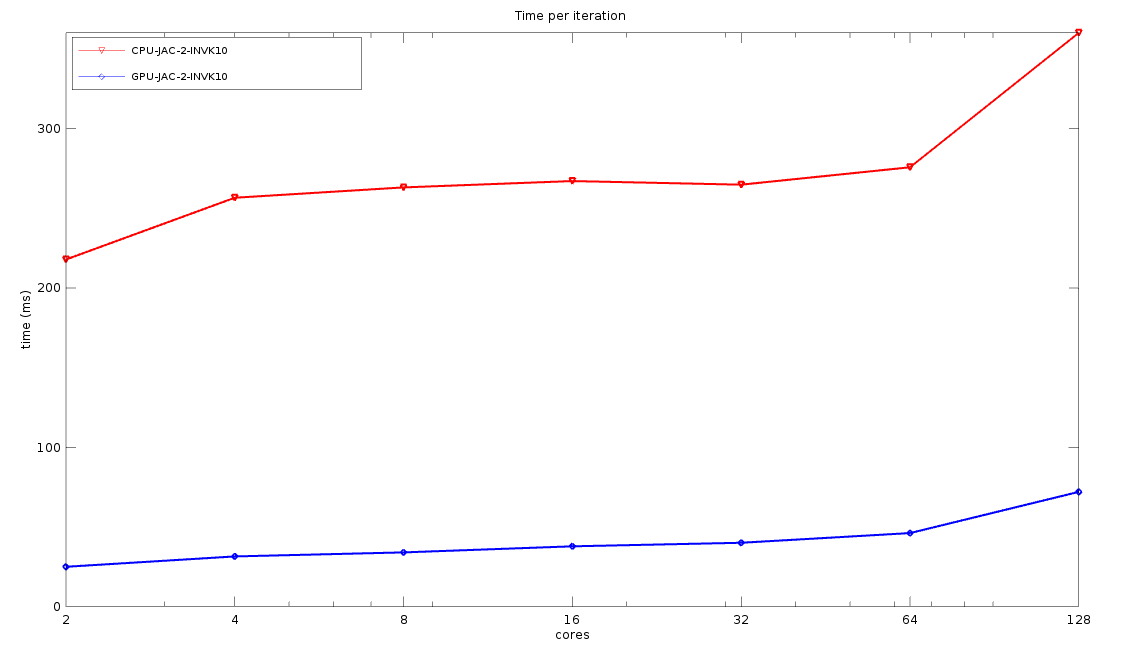
\includegraphics[width=0.9\textwidth]{graf_time_per_it3a.png}
\caption{Jacobi-INVK, time per iteration\label{fig:time_per_it_a}}
\end{figure}

\begin{figure}[h!]
\centering
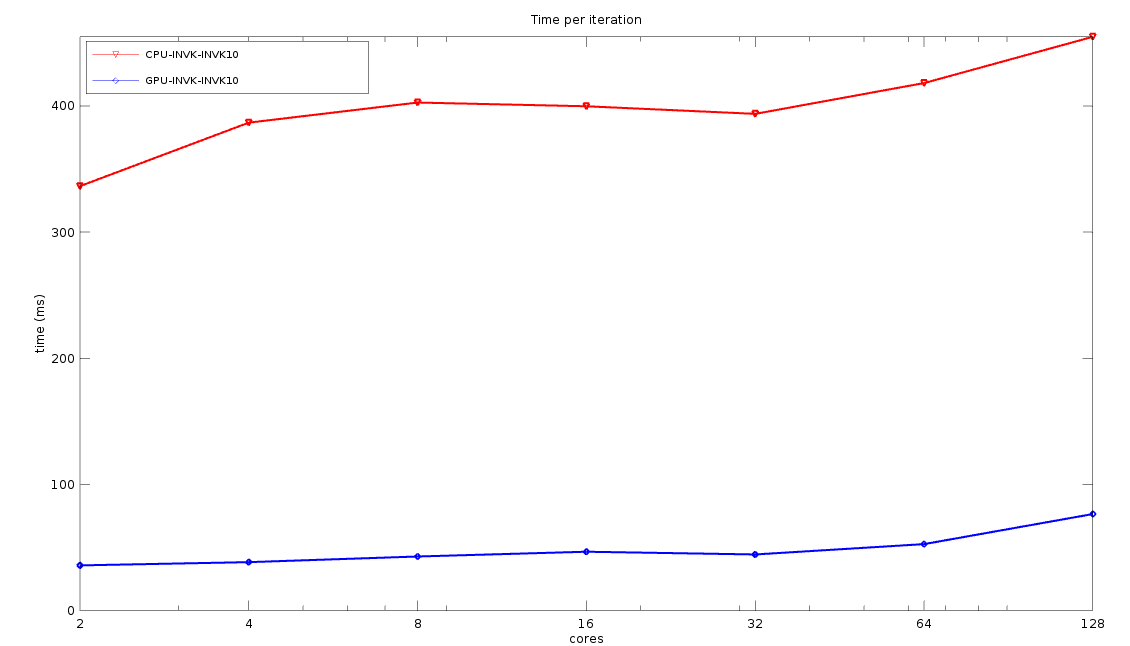
\includegraphics[width=0.9\textwidth]{graf_time_per_it3b.png}
\caption{INVK-INVK, time per iteration\label{fig:time_per_it_b}}
\end{figure}

In Figures~\ref{fig:time_per_it_a} and~\ref{fig:time_per_it_b}
we see that the time per iteration with the GPUs has a very flat profile between 2
and 64 nodes; this reflects a very good weak scalability within each
iteration of the method.

 However to translate this into a flat
solution time it is necessary that the number of iterations remains
constant; let us then turn our attention to the Tables~\ref{gpu-invk}
and~\ref{gpu-jac}. In the tables, we show 
respectively the number of processing elements (CPU cores or GPU
devices), the number of levels in the multilevel hierarchy, the time
for setup in seconds, then the time to solution and time per iteration
(in seconds and milliseconds), for CPUs and GPUs respectively; finally,
we show the solution speedup. The time 
to setup is essentially identical, because  almost all the
setup process is currently executed  on CPUs; in all cases, the number
of iterations to convergence is identical on CPUs and GPUs. 

There are two lines for the tests at 128 devices in each table. 
The first line is obtained by letting the aggregation algorithm run with
default arguments; in this case the preconditioner uses a hierarchy
with 5 levels and achieves a number of iterations equal to or less than
that for 32 and 64 devices, but because there are 5 levels, the time
per iteration deteriorates.  In the second line, we force the
preconditioner to use 4 levels, in which case the time per iteration
remains essentially constant on the GPU and very close on the CPU, but
the number of iterations increases. In both
configurations the best solution time on the GPU is obtained with 4
levels, whereas the CPU version is faster with 5 levels. 

In summary, the aggregation algorithm is capable of obtaining very
good algorithmic scalability, but in some cases at the expense of time
per iteration, so that it does not necessarily correspond to the best 
solution time. 
Additional work will be required to design aggregation
strategies capable of obtaining a better trade-off with as little user
intervention as possible; some possible directions are outlined
in~\cite{bcm-toms}.  




\iffalse
\begin{table}[h!]
\centering
\caption{Numerical results for CG + ML preconditioner, runs on CPUs, with 1 sweep of BJAC(INVK) as smoother on inner levels.}
\label{cpu-invk}

\begin{tabular}{rrrrrrr}
% \multicolumn{1}{l}{np} & \multicolumn{1}{l}{levels} &   \multicolumn{1}{l}{Iters} & \multicolumn{1}{l}{\begin{tabular}[c]{@{}l@{}}Prec    \\  
%  time (s)\end{tabular}} &
%                           \multicolumn{1}{l}{\begin{tabular}[c]{@{}l@{}}Solve  \\  
% Time (s)\end{tabular}} &
%                          \multicolumn{1}{l}{\begin{tabular}[c]{@{}l@{}}Time per \\ 
% Iteration (ms)\end{tabular}} & \multicolumn{1}{l}{\begin{tabular}[c]{@{}l@{}}Total  \\   Time (s)\end{tabular}} \\ \hline
NP  & Levels & Iters & Tsetup & Tsolve & T/iter & Ttotal \\
    &        &       & (s)    & (s)    & (ms)   & (s)    \\
\hline
1   & 4       & 14  & 17.74 & 4.42  & 320      & 22.15   \\
2   & 4       & 15  & 19.43 & 5.05  & 340      & 24.47   \\
4   & 4       & 18  & 21.85 & 6.96  & 390      & 28.81   \\
8   & 4       & 20  & 28.32 & 8.05  & 400      & 36.37   \\
16  & 4       & 24  & 26.38 & 9.59  & 400      & 35.98   \\
32  & 4       & 29  & 23.52 & 11.42 & 390      & 34.93   \\
64  & 4       & 34  & 29.61 & 14.21 & 420      & 43.82   \\
128 & 5       & 29  & 28.39 & 13.19 & 450      & 41.58    \\
\hline
\end{tabular}
\end{table}

\begin{table}[h!]
\centering
\caption{Numerical results for CG + ML preconditioner, runs on GPUs, with 1 sweep of BJAC(INVK) as smoother on inner levels.}
\label{gpu-invk}

\begin{tabular}{rrrrrrrr}
% \multicolumn{1}{l}{np} & \multicolumn{1}{l}{levels} & \multicolumn{1}{l}{It} & \multicolumn{1}{l}{\begin{tabular}[c]{@{}l@{}}Prec    \\   time (s)\end{tabular}} & \multicolumn{1}{l}{\begin{tabular}[c]{@{}l@{}}Solve  \\  Time (s)\end{tabular}} & \multicolumn{1}{l}{\begin{tabular}[c]{@{}l@{}}Time per \\ Iteration (ms)\end{tabular}} & \multicolumn{1}{l}{\begin{tabular}[c]{@{}l@{}}Total  \\   Time (s)\end{tabular}} & \multicolumn{1}{l}{\begin{tabular}[c]{@{}l@{}}Speed up\\ cpu/gpu\end{tabular}} \\ \hline
NP  & Levels & Iters & Tsetup & Tsolve & T/iter & Ttotal & Speedup\\
    &        &       & (s)    & (s)    & (ms)   & (s)   &  \\
\hline
1   & 4       & 14  & 18.80 & 0.45 & 30   & 19.24& 9.92  \\
2   & 4       & 15  & 20.55 & 0.54 & 40   & 21.09& 9.40  \\
4   & 4       & 18  & 22.84 & 0.69 & 40   & 23.54& 10.08 \\
8   & 4       & 20  & 29.18 & 0.86 & 40   & 30.03& 9.40  \\
16  & 4       & 24  & 27.38 & 1.12 & 50   & 28.50& 8.57  \\
32  & 4       & 29  & 23.74 & 1.29 & 40   & 25.02& 8.85  \\
64  & 4       & 34  & 30.53 & 1.79 & 50   & 32.32& 7.94  \\
128 & 5       & 29  & 29.48 & 2.22 & 80   & 31.70& 5.94  \\
\hline
\end{tabular}
\end{table}

\begin{table}[h!]
\centering
\caption{Numerical results for CG + ML preconditioner, runs on CPUs, with 2 sweeps of JACOBI as smoother on inner levels.}
\label{cpu-jac}

\begin{tabular}{rrrrrrr}
% \multicolumn{1}{l}{np} & \multicolumn{1}{l}{levels} & \multicolumn{1}{l}{It} & \multicolumn{1}{l}{\begin{tabular}[c]{@{}l@{}}Prec    \\   time (s)\end{tabular}} & \multicolumn{1}{l}{\begin{tabular}[c]{@{}l@{}}Solve  \\  Time (s)\end{tabular}} & \multicolumn{1}{l}{\begin{tabular}[c]{@{}l@{}}Time per \\ Iteration (s)\end{tabular}} & \multicolumn{1}{l}{\begin{tabular}[c]{@{}l@{}}Total  \\   Time (s)\end{tabular}} \\ \hline
NP  & Levels & Iters & Tsetup & Tsolve & T/iter & Ttotal \\
    &        &       & (s)    & (s)    & (ms)   & (s)    \\
\hline
1   & 4       & 19  & 2.83  & 3.76  & 200   & 6.59    \\
2   & 4       & 21  & 3.65  & 4.57  & 220   & 8.23    \\
4   & 4       & 20  & 4.21  & 5.13  & 260   & 9.35    \\
8   & 4       & 25  & 4.75  & 6.58  & 260   & 11.33   \\
16  & 4       & 27  & 4.97  & 7.21  & 270   & 12.18   \\
32  & 4       & 31  & 4.88  & 8.21  & 260   & 13.09   \\
64  & 4       & 37  & 5.79  & 10.20 & 280   & 16.00   \\
128 & 5       & 31  & 6.72  & 11.16 & 360   & 17.88  \\
\hline
\end{tabular}
\end{table}

\begin{table}[h!]
\centering
\caption{Numerical results for CG + ML preconditioner, runs on GPUs, with 2 sweeps of JACOBI as smoother on inner levels.}
\label{gpu-jac}
\begin{tabular}{rrrrrrrr}
% \multicolumn{1}{l}{np} & \multicolumn{1}{l}{levels} & \multicolumn{1}{l}{It} & \multicolumn{1}{l}{\begin{tabular}[c]{@{}l@{}}Prec    \\   time (s)\end{tabular}} & \multicolumn{1}{l}{\begin{tabular}[c]{@{}l@{}}Solve  \\  Time (s)\end{tabular}} & \multicolumn{1}{l}{\begin{tabular}[c]{@{}l@{}}Time per \\ Iteration (s)\end{tabular}} & \multicolumn{1}{l}{\begin{tabular}[c]{@{}l@{}}Total  \\   Time (s)\end{tabular}} & \multicolumn{1}{l}{\begin{tabular}[c]{@{}l@{}}Speed up\\ cpu/gpu\end{tabular}} \\ \hline
NP  & Levels & Iters & Tsetup & Tsolve & T/iter & Ttotal & Speedup\\
    &        &       & (s)    & (s)    & (ms)   & (s)   &  \\
\hline
1   & 4       & 19  & 3.13  & 0.40 & 20   & 3.53 & 9.39  \\
2   & 4       & 21  & 4.06  & 0.52 & 20   & 4.59 & 8.73  \\
4   & 4       & 20  & 4.65  & 0.63 & 30   & 5.28 & 8.16  \\
8   & 4       & 25  & 5.20  & 0.85 & 30   & 6.05 & 7.74  \\
16  & 4       & 27  & 5.39  & 1.02 & 40   & 6.42 & 7.06  \\
32  & 4       & 31  & 5.35  & 1.24 & 40   & 6.59 & 6.61  \\
64  & 4       & 37  & 6.25  & 1.71 & 50   & 7.96 & 5.98  \\ 
128 & 5       & 31  & 7.19  & 2.23 & 70   & 9.43 & 5.00  \\
\hline
\end{tabular}
\end{table}

\else

\begin{table}[h!]
\centering
\begin{tabular}{rrrrrrrrr}
% \multicolumn{1}{l}{np} & \multicolumn{1}{l}{levels} &
% \multicolumn{1}{l}{It} &
% \multicolumn{1}{l}{\begin{tabular}[c]{@{}l@{}}Prec    \\   time
% (s)\end{tabular}} &
% \multicolumn{1}{l}{\begin{tabular}[c]{@{}l@{}}Solve  \\  Time
% (s)\end{tabular}} &
% \multicolumn{1}{l}{\begin{tabular}[c]{@{}l@{}}Time per \\ Iteration
% (ms)\end{tabular}} &
% \multicolumn{1}{l}{\begin{tabular}[c]{@{}l@{}}Total  \\   Time
% (s)\end{tabular}} &
% \multicolumn{1}{l}{\begin{tabular}[c]{@{}l@{}}Speed up\\
% cpu/gpu\end{tabular}} \\ \hline
    &        &       &        & \multicolumn{2}{c}{CPU} & \multicolumn{2}{c}{GPU} & \\
NP  & Levels & Iters & Tsetup & Tsolve & T/iter  & Tsolve & T/iter  & Speedup\\
    &        &       & (s)    & (s)    & (ms)    & (s)    & (ms)    & GPU/CPU \\
\hline
1   & 4       & 14  & 18.80 & 4.42  & 320    & 0.45 & 30   &  9.92  \\
2   & 4       & 15  & 20.55 & 5.05  & 340    & 0.54 & 40   &  9.40  \\
4   & 4       & 18  & 22.84 & 6.96  & 390    & 0.69 & 40   &  10.08 \\
8   & 4       & 20  & 29.18 & 8.05  & 400    & 0.86 & 40   &  9.40  \\
16  & 4       & 24  & 27.38 & 9.59  & 400    & 1.12 & 50   &  8.57  \\
32  & 4       & 29  & 23.74 & 11.42 & 390    & 1.29 & 40   &  8.85  \\
64  & 4       & 34  & 30.53 & 14.21 & 420    & 1.79 & 50   &  7.94  \\
128 & 5       & 29  & 29.48 & 13.19 & 450    & 2.22 & 80   &  5.94  \\
\hline
128 & 4       & 43  & 29.48 & 19.32 & 450    & 2.18 & 51   &  8.85  \\
\hline
\end{tabular}
\caption{Weak Scalability,  CG + ML preconditioner,  with 1 sweep of BJAC(INVK) smoother on inner levels.\label{gpu-invk}}
\end{table}


\begin{table}[h!]
\centering
\begin{tabular}{rrrrrrrrrrr}
% \multicolumn{1}{l}{np} & \multicolumn{1}{l}{levels} & \multicolumn{1}{l}{It} & \multicolumn{1}{l}{\begin{tabular}[c]{@{}l@{}}Prec    \\   time (s)\end{tabular}} & \multicolumn{1}{l}{\begin{tabular}[c]{@{}l@{}}Solve  \\  Time (s)\end{tabular}} & \multicolumn{1}{l}{\begin{tabular}[c]{@{}l@{}}Time per \\ Iteration (s)\end{tabular}} & \multicolumn{1}{l}{\begin{tabular}[c]{@{}l@{}}Total  \\   Time (s)\end{tabular}} & \multicolumn{1}{l}{\begin{tabular}[c]{@{}l@{}}Speed up\\ cpu/gpu\end{tabular}} \\ \hline
    &        &       &        & \multicolumn{2}{c}{CPU} &\multicolumn{2}{c}{GPU} & \\
NP  & Levels & Iters & Tsetup & Tsolve & T/iter & Tsolve & T/iter  & Speedup\\
    &        &       & (s)    & (s)    & (ms)   & (s)    & (ms)    & GPU/CPU \\
\hline
1   & 4       & 19  & 3.13  & 3.76  & 200 & 0.40 & 20   & 9.39  \\
2   & 4       & 21  & 4.06  & 4.57  & 220 & 0.52 & 20   & 8.73  \\
4   & 4       & 20  & 4.65  & 5.13  & 260 & 0.63 & 30   & 8.16  \\
8   & 4       & 25  & 5.20  & 6.58  & 260 & 0.85 & 30   & 7.74  \\
16  & 4       & 27  & 5.39  & 7.21  & 270 & 1.02 & 40   & 7.06  \\
32  & 4       & 31  & 5.35  & 8.21  & 260 & 1.24 & 40   & 6.61  \\
64  & 4       & 37  & 6.25  & 10.20 & 280 & 1.71 & 50   & 5.98  \\ 
128 & 5       & 31  & 7.19  & 11.16 & 360 & 2.23 & 70   & 5.00  \\
\hline
128 & 4       & 46  & 7.00  & 14.05 & 305 & 2.04 & 44   & 6.88  \\
\hline
\end{tabular}
\caption{Weak Scalability,  CG + ML preconditioner,  with 2 sweeps of JACOBI smoother on inner levels.\label{gpu-jac}}
\end{table}
\fi

% When GPUs are used, the last column shows the speed-up of the solver
% phase on the gpu with respect to the cpu solve time.
The GPU/CPU speed-up achieves a maximum value of 10 in the case of 8
processes and it achieves a value between  5 and 9  with 128
processes. The  increasing number of levels leads to a decrease in
the size of the coarsest level matrix which affects performance for
two reasons, first because the matrices at the coarse level are too
small to make good use of the GPU device computational power, and also
because the communication to computation ratio gets worse.


% \begin{figure}[h!]
% \caption{Time per iteration}
% \centering
% 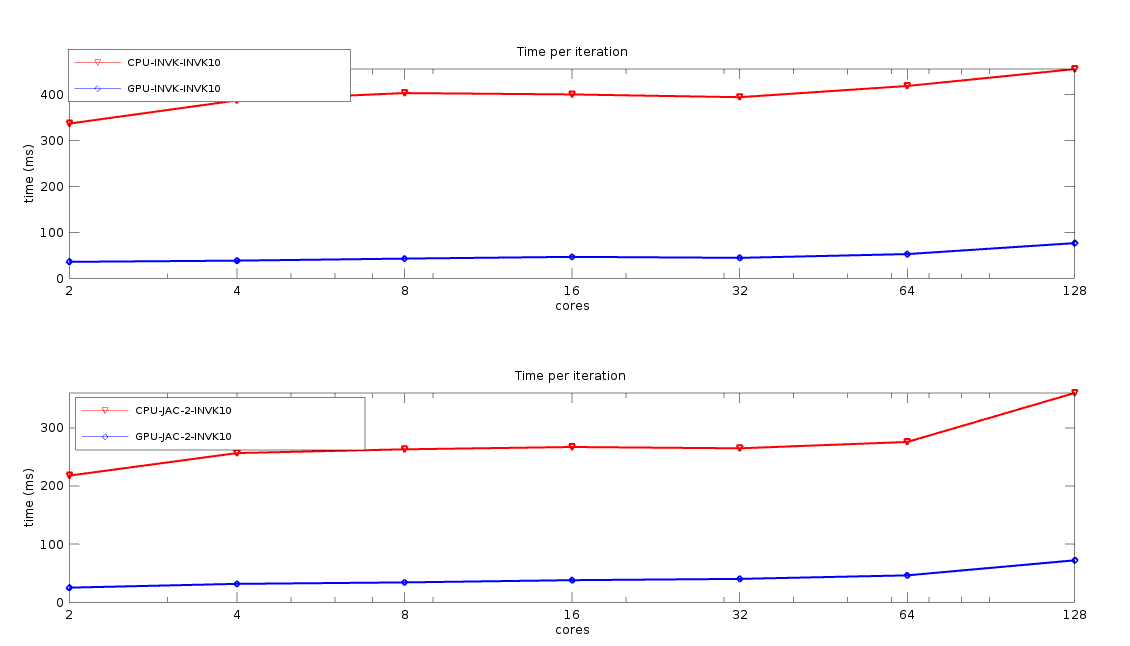
\includegraphics[width=1\textwidth]{time_per_it.png}
% \label{fig:time_per_it}
% \end{figure}


% \begin{figure}
% \begin{center}
% 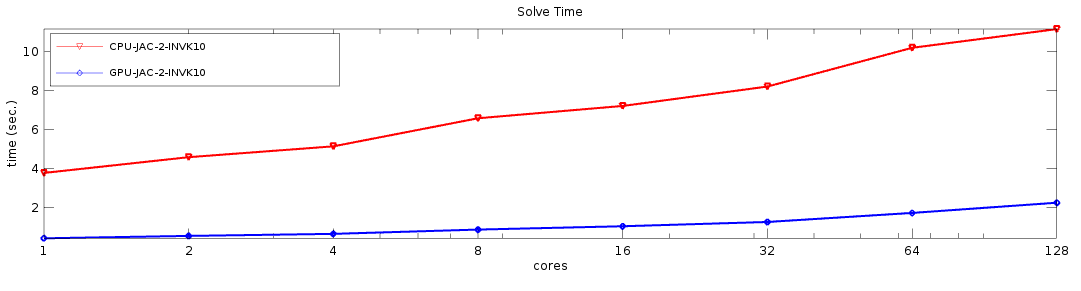
\includegraphics[width=.9\textwidth]{graf_jac2.png}
% \end{center}
% \caption{JAC2-INVK}
% \end{figure}


%%%%%%% ACK
%\subsection*{Acknowledgments}\label{sec:Acknowledgments}


%
% ---- Bibliography ----
%
\bibliographystyle{splncs03}
\bibliography{europar}

% \begin{thebibliography}{6}
% %

% \bibitem {}


% \end{thebibliography}
\end{document}
